% Short IEEE-format extract of the paper (title, abstract, introduction and
% proposed method) for review by the guide. It states the proposed work only
% and contains no experimental results.
\documentclass[conference]{IEEEtran}
\IEEEoverridecommandlockouts

\usepackage{cite}
\usepackage{amsmath,amssymb,amsfonts}
\usepackage{graphicx}
\usepackage{textcomp}
\usepackage{xcolor}
\usepackage{url}
\usepackage{tikz}
\usetikzlibrary{positioning,arrows.meta,fit}

\begin{document}

\title{ENSO-Aware Adversarial Forecasting: A Unified WGAN-GP Framework for Extreme-Aware Imputation and Forecasting of Heatwave Days in Regional Temperature Time Series}

\author{
\IEEEauthorblockN{Melvin Immanuel G}
\IEEEauthorblockA{\textit{Department of Mathematics} \\
\textit{School of Advanced Sciences} \\
\textit{Vellore Institute of Technology}\\
Chennai, India}
\and
\IEEEauthorblockN{Nainor Selvan G}
\IEEEauthorblockA{\textit{Department of Mathematics} \\
\textit{School of Advanced Sciences} \\
\textit{Vellore Institute of Technology}\\
Chennai, India}
\and
\IEEEauthorblockN{Prof.\ Dr.\ Kalyani Desikan}
\IEEEauthorblockA{\textit{Department of Mathematics} \\
\textit{School of Advanced Sciences} \\
\textit{Vellore Institute of Technology}\\
Chennai, India}
}

\maketitle

\begin{abstract}
Weather and climate time series are simultaneously non-stationary, gap-prone, and characterized by
rare but high-impact extreme events such as heatwaves. Over India, the frequency and persistence of
heatwaves are further modulated by the El Ni\~{n}o--Southern Oscillation (ENSO), so that the days of
greatest practical consequence cluster in El Ni\~{n}o-affected seasons. Existing generative adversarial
network (GAN) approaches to this domain address imputation and forecasting as separate problems and
ignore large-scale climate drivers such as ENSO. We propose a unified adversarial framework in which a
single ENSO-conditioned generator performs both missing-data imputation and multi-step forecasting of
heatwave days for a regional temperature series, trained with a Wasserstein GAN with gradient penalty
(WGAN-GP) objective augmented by a generalized-extreme-value-inspired exceedance-weighted loss term.
The generator and critic are conditioned on a causally lagged Oceanic Ni\~{n}o Index, so that the model
can learn how the likelihood and intensity of heatwave days shift with the ENSO phase. The framework is
evaluated on ERA5-Land daily reanalysis for Chennai, India, under a temporally held-out protocol, with
continuous-value metrics (RMSE, MAE, R\textsuperscript{2}, extreme-tail RMSE) and event-level metrics
(probability of detection, false alarm ratio, critical success index) aligned to the India
Meteorological Department heatwave definition and reported separately for El Ni\~{n}o, La Ni\~{n}a and
neutral periods.
\end{abstract}

\begin{IEEEkeywords}
generative adversarial networks, WGAN-GP, time series imputation, weather forecasting, extreme value
theory, heatwave prediction, El Ni\~{n}o--Southern Oscillation, ERA5-Land
\end{IEEEkeywords}

\section{Introduction}

Missing observations and the need to project future states are two persistent, related challenges in
regional climate time series analysis. Sensor outages, transmission loss, and irregular station
coverage all produce gaps that must be filled before a series can be analyzed or modeled, while
early-warning systems require genuine forecasts of future values. Both problems are compounded when the
quantity of interest is prone to extreme excursions: temperature series in heatwave-prone regions such
as peninsular India are dominated in aggregate by smooth seasonal cycles, yet the events of greatest
practical consequence---heatwaves---sit in the tail of the distribution, precisely where models trained
under a mean-squared-error objective are least reliable.

Heatwave occurrence over India is not stationary from year to year. ENSO, the dominant mode of
interannual climate variability in the tropical Pacific \cite{trenberth1997definition,mcphaden2006enso},
influences Indian surface temperature through atmospheric teleconnections, and the frequency and
duration of Indian heatwaves have been linked to El Ni\~{n}o conditions in the central and eastern
Pacific \cite{rohini2016variability,ratnam2016anatomy}. A model that imputes or forecasts temperature
without access to the ENSO state must treat El Ni\~{n}o and La Ni\~{n}a years as draws from a single
distribution, and is therefore likely to under-predict exactly the heatwave days that cluster in
El Ni\~{n}o-affected seasons.

GANs \cite{goodfellow2014generative} have been applied to both imputation \cite{luo2018multivariate}
and forecasting \cite{bihlo2021generative} of weather data, and extreme-value-aware objectives improve
tail fidelity in both non-adversarial \cite{ding2019modeling} and adversarial
\cite{huster2021pareto,bhatia2021exgan,boulaguiem2022modeling} settings. However, no existing framework
combines imputation and forecasting within a single adversarially-trained generator for a region-scale
series, no extreme-value-aware GAN has been applied to city-scale temperature in a heatwave-prone
setting such as India, and none conditions on the ENSO state that modulates heatwave risk. A closely
related study on Chennai heatwave classification \cite{choudary2025comparative} names time series GANs
as a plausible, unexplored strategy for the class imbalance of rare heatwave events, but does not pursue
it.

The proposed work makes the following contributions:
\begin{enumerate}
    \item A unified adversarial framework in which a single generator performs both interior-gap
    imputation and multi-step forecasting, differing only in where the reconstruction mask falls within
    a training window.
    \item ENSO conditioning of both the generator and the WGAN-GP critic on a causally lagged Oceanic
    Ni\~{n}o Index (ONI), so that imputed and forecast heatwave days are generated conditionally on the
    El Ni\~{n}o, La Ni\~{n}a or neutral state of the tropical Pacific.
    \item A generalized-extreme-value-inspired exceedance-weighted loss that makes the reconstruction
    objective explicitly sensitive to heatwave behavior, combined with a WGAN-GP adversarial objective
    \cite{arjovsky2017wasserstein,gulrajani2017improved}.
    \item A temporally held-out evaluation protocol that reports continuous and event-level
    (POD/FAR/CSI) metrics stratified by ENSO phase, for direct comparability with classification-style
    heatwave studies.
\end{enumerate}

\section{Proposed Methodology}

\begin{figure}[t]
\centering
\resizebox{\columnwidth}{!}{% Framework diagram shared by main.tex and snippet.tex (requires tikz with
% the positioning, arrows.meta and fit libraries).
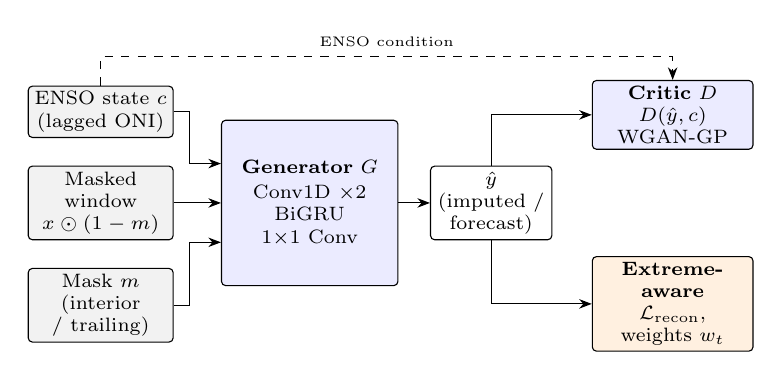
\begin{tikzpicture}[
  font=\scriptsize,
  >={Stealth[length=1.6mm]},
  node distance=3.5mm and 4mm,
  box/.style={draw, rounded corners=1.5pt, align=center, minimum height=6.5mm, inner sep=2pt, fill=white},
  inp/.style={box, fill=gray!10, text width=17mm},
  net/.style={box, fill=blue!8, text width=19mm},
  loss/.style={box, fill=orange!12, text width=19mm}
]
  % Inputs
  \node[inp] (c)   {ENSO state $c$\\(lagged ONI)};
  \node[inp, below=of c] (x)   {Masked window\\$x \odot (1-m)$};
  \node[inp, below=of x] (m)   {Mask $m$\\(interior / trailing)};

  % Generator
  \node[net, right=6mm of x, text width=21mm, minimum height=21mm] (G)
    {\textbf{Generator $G$}\\[1pt] Conv1D $\times 2$\\ BiGRU\\ $1{\times}1$ Conv};

  % Output
  \node[box, right=of G, text width=14mm] (yhat) {$\hat{y}$\\(imputed /\\forecast)};

  % Critic and loss
  \node[net, above right=2mm and 5mm of yhat] (D) {\textbf{Critic $D$}\\$D(\hat{y}, c)$\\WGAN-GP};
  \node[loss, below right=2mm and 5mm of yhat] (L) {\textbf{Extreme-aware}\\$\mathcal{L}_{\mathrm{recon}}$, weights $w_t$};

  % Arrows
  \draw[->] (c.east) -- ++(2mm,0) |- ([yshift=5mm]G.west);
  \draw[->] (x.east) -- (G.west);
  \draw[->] (m.east) -- ++(2mm,0) |- ([yshift=-5mm]G.west);
  \draw[->] (G) -- (yhat);
  \draw[->] (yhat.north) |- (D.west);
  \draw[->] (yhat.south) |- (L.west);
  \coordinate (top) at ([yshift=3mm]D.north);
  \draw[->, dashed] (c.north) |- node[pos=0.75, above, font=\tiny] {ENSO condition} (top) -- (D.north);
\end{tikzpicture}
}
\caption{Proposed ENSO-aware framework. A single generator receives a masked temperature window, the
mask, and the lagged ENSO state, and fills either an interior gap (imputation) or the trailing $k$ days
(forecasting). It is trained with an ENSO-conditioned WGAN-GP critic and an extreme-aware weighted
reconstruction loss.}
\label{fig:framework}
\end{figure}

\subsection{Data}

Daily 2\,m air temperature and auxiliary variables are taken from the ERA5-Land reanalysis
\cite{munozsabater2021era5land} via Google Earth Engine \cite{gorelick2017gee} for Chennai
(13.08\,\textdegree N, 80.23\,\textdegree E) and split chronologically into training, validation and
test periods; scaling parameters and thresholds are fit on the training period only. The ENSO state is
the monthly NOAA ONI \cite{noaa_oni}, the three-month running mean of ERSSTv5 Ni\~{n}o-3.4 SST anomalies
\cite{huang2017ersstv5}; months are labeled El Ni\~{n}o (La Ni\~{n}a) when the ONI is at or above
$+0.5\,^{\circ}$C (at or below $-0.5\,^{\circ}$C) for at least five consecutive overlapping seasons.
Because the ONI is a centered mean, the model uses only the value published before the start of each
window (a lag of $\ell \geq 2$ months), keeping the forecasts operationally causal. Heatwave days follow
the India Meteorological Department criterion for coastal stations \cite{imd2024heatwave}: a departure
of at least $4.5\,^{\circ}$C from the calendar-day normal of the daily maximum, with an actual maximum of
at least $37\,^{\circ}$C.

\subsection{Unified Masked Reconstruction}

Given a window of length $W$ and a binary mask $m \in \{0,1\}^W$, the generator fills the hidden
positions. An interior masked span is an imputation task; a trailing span of $k$ steps is a $k$-step
forecast. The mask type, position and length are resampled for every training window, so that the
model is never trained on the exact segments it is scored on. Each window carries a conditioning
vector $c$ holding the lagged ONI, and the generator learns
$p(y_{\mathcal{M}} \mid y_{\bar{\mathcal{M}}}, c)$, the distribution of the hidden values given the
observed context and the ENSO state.

\subsection{Architecture and Adversarial Objective}

The generator consists of two 1-D convolutional layers (kernel size 5) over the masked values, the mask
indicator and the ENSO channels, followed by a bidirectional GRU and a $1\times1$ convolution. The
critic is convolutional and conditional \cite{mirza2014conditional}: it scores a completed window
together with $c$, so that it judges whether a heatwave sequence is realistic for the given ENSO state.
It is trained with the WGAN-GP loss \cite{gulrajani2017improved}
\begin{equation}
\mathcal{L}_D = \mathbb{E}\big[D(\hat{x}, c)\big] - \mathbb{E}\big[D(x, c)\big]
+ \gamma\, \mathbb{E}\Big[\big(\lVert \nabla_{\tilde{x}} D(\tilde{x}, c) \rVert_2 - 1\big)^2\Big],
\end{equation}
where $\hat{x}$ is the generator-completed window and $\tilde{x}$ a random interpolation between real
and completed windows.

\subsection{Extreme-Value-Aware Loss}

Following the extreme value loss of Ding et al.~\cite{ding2019modeling}, masked positions are weighted
by their exceedance over the heatwave threshold $\tau_t$:
\begin{equation}
w_t = 1 + \lambda \cdot \max\!\left(0, \frac{y_t - \tau_t}{\sigma}\right),
\end{equation}
\begin{equation}
\mathcal{L}_{\text{recon}} = \frac{1}{|\mathcal{M}|}\sum_{t \in \mathcal{M}} w_t (\hat y_t - y_t)^2,
\end{equation}
where $\sigma$ is the training standard deviation and $\lambda$ sets the emphasis on extremes. The
generator minimizes
\begin{equation}
\mathcal{L}_G = -\mathbb{E}\big[D(\hat{x}, c)\big] + \beta \, \mathcal{L}_{\text{recon}},
\end{equation}
with $\beta$ chosen so that the two terms are of comparable magnitude. Training windows are sampled so
that the three ENSO phases are equally represented in each mini-batch.

\subsection{Evaluation Plan}

The model is compared with ARIMA, SARIMA and KNN baselines fit on the same observed context, and with
ablations that remove the adversarial term, remove the ENSO conditioning, or shuffle the ONI across
years. Reported metrics are RMSE, MAE, R\textsuperscript{2}, extreme-tail RMSE, and the event-level
probability of detection, false alarm ratio and critical success index for heatwave days, over the full
test period and separately for El Ni\~{n}o, La Ni\~{n}a and neutral months. Differences in forecast
error are tested with the Diebold--Mariano test \cite{diebold1995comparing}.

\bibliographystyle{IEEEtran}
\bibliography{references}

\end{document}
